\documentclass[12pt,fullpage,letterpaper]{article}

\newenvironment{proof}{\noindent{\bf Proof:}}{\qed\bigskip}

\newtheorem{theorem}{Theorem}
\newtheorem{corollary}{Corollary}
\newtheorem{lemma}{Lemma} 
\newtheorem{claim}{Claim}
\newtheorem{fact}{Fact}
\newtheorem{definition}{Definition}
\newtheorem{assumption}{Assumption}
\newtheorem{observation}{Observation}
\newtheorem{example}{Example}
\newcommand{\qed}{\rule{5pt}{7pt}}

\newcommand{\assignment}[4]{
\thispagestyle{plain} 
\newpage
\setcounter{page}{1}
\noindent
\begin{center}
\framebox{ \vbox{ \hbox to 7in
{\bf CS466: Introduction to Bioinformatics \hfill #1}
\vspace{4mm}
\hbox to 6.28in
{\hspace{2.5in}\large\mbox{Problem Set #2}}
\vspace{4mm}
\hbox to 6.28in
{{\it Handed out: #3 \hfill Due: #4}}
}}
\end{center}
}


\newcommand{\handout}[3]{
\thispagestyle{plain} 
\newpage
\setcounter{page}{1}
\noindent
\begin{center}
\framebox{ \vbox{ \hbox to 6.28in
{\bf CS466: Introduction to Bioinformatics \hfill #1}
\vspace{4mm}
\hbox to 6.28in
{\hspace{2.5in}\large\mbox{#2}}
\vspace{4mm}
\hbox to 6.28in
{{\it Handed Out: #3 \hfill Name (NetID): \rule[-2pt]{4cm}{0.1pt} }}
}}
\end{center}
}


\newcommand{\assgsoln}[4]{
\thispagestyle{plain} 
\newpage
\setcounter{page}{1}
\noindent
\begin{center}
\framebox{ \vbox{ \hbox to 6.28in
{\bf CCS466: Introduction to Bioinformatics n \hfill #1}
\vspace{4mm}
\hbox to 6.28in
{\hspace{2.5in}\large\mbox{Problem Set #2 Solutions}}
\vspace{4mm}
\hbox to 6.28in
{{\it Handed Out: #3 \hfill Handed In: #4}}
}}
\end{center}
}


\newenvironment{algorithm}
{\begin{center}
\begin{tabular}{|l|}
\hline
\begin{minipage}{1in}
\begin{tabbing}
\quad\=\qquad\=\qquad\=\qquad\=\qquad\=\qquad\=\qquad\=\kill}
{\end{tabbing}
\end{minipage} \\
\hline
\end{tabular}
\end{center}}

\def\Comment#1{\textsf{\textsl{$\langle\!\langle$#1\/$\rangle\!\rangle$}}}




\oddsidemargin 0in
\evensidemargin 0in
\textwidth 6.5in
\topmargin -0.5in
\textheight 9.0in

\usepackage{hyperref}
\usepackage{float}
\usepackage{pdfpages}
\usepackage{textcomp}
\usepackage{mathtools}
\usepackage{algorithm}
\usepackage{array}
\usepackage{tabu}
\usepackage{changepage}
\usepackage{amsmath}
\usepackage{amssymb}
\usepackage[noend]{algpseudocode}
\usepackage{graphicx,url,epstopdf}
\usepackage{xcolor}
\usepackage{color,soul}
\usepackage{tabularray}
\usepackage {tikz}
\usetikzlibrary {positioning}
\makeatletter
\def\BState{\State\hskip-\ALG@thistlm}
\makeatother
\sloppy
\usepackage{colortbl}


\setul{0.5ex}{0.3ex}
\setulcolor{blue}

\newcommand\tab[1][1cm]{\hspace*{#1}}

\begin{document}

\assignment{Name: Payal Mantri \hspace{5cm}}{4}{November 9, 2022}{Nov 17, 2022}
% Fill in the above, for example, as follows:
% \solution{Joe Smith}{\today}{1}{Fall 2012}

\pagestyle{myheadings}  % Leave this command alone

\noindent\emph{Instructions:} This homework assignment consists of two questions worth a total of 50 points. 
% In addition, there is a bonus question worth an additional 5 points.
% These questions are based on the material covered in Lectures 13 to 18.
\textbf{Do not forget to write your name at the top!}

\begin{enumerate}
\item[1.] \textbf{Assembly I} [25 points]

\begin{enumerate}
% i can use more than 2 letters too,
\item[a.] Compute for each permutation of the set $S$  = \{ABB, BAB, ABA\} the corresponding shortest common superstring (SCS) respecting the order prescribed by the permutation. Indicate the permutation(s) with overall shortest common superstring. [10~points]

\emph{Hint:} There are $3! = 6$ permutations of $S$.

\fbox{\parbox{\linewidth}{
\setulcolor{red}
\begin{enumerate}
    \item $S$  = \{ABB, \ul{B}AB, \ul{AB}A\} \\
 $   SCS(S) = ABBABA \Rightarrow length = 6$ \\
    
    \item $S$  = \{ABB, ABA , \ul{BA}B \} \\
   $ SCS(S) = ABBABAB \Rightarrow length = 7$\\
   
    \item $S$  = \{BAB, \ul{AB}B , ABA \} \\
   $ SCS(S) = BABBABA \Rightarrow length = 7$ \\

       \item $S$  = \{BAB, \ul{AB}A , \ul{A}BB \} \\
   $ SCS(S) = BABABB \Rightarrow length = 6$ \\
   
    \item $S$  = \{ABA, \ul{A}BB , \ul{B}AB \} \\
    $SCS(S) = ABABBAB \Rightarrow length = 7$ \\
    \item $S$  = \{ABA, \ul{BA}B , \ul{AB}B \} \\
    $SCS(S) = ABABB \Rightarrow length =5$ \\
  
\end{enumerate}

\textbf{Overall shortest common substring $SCS(S) = ABABB \Rightarrow length =5$ }
\vspace{1cm}
}}
\clearpage
\item[b.] Consider the same set $S$  = \{ABB, BAB, ABA\} as in the previous question. Use the greedy heuristic to approximate the SCS problem. Give the edge-weighted directed graph for each step of the greedy heuristic. In the case of multiple edges with the same maximum weight, enumerate all solutions. [10~points]


\begin {center}
\begin{tabular}{|c|c|c|}
   
\hline
\SetCell[r=4]{}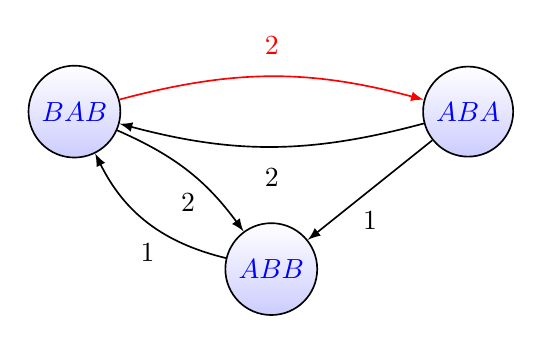
\begin{tikzpicture}[-latex ,auto ,node distance =2 cm and 2.5cm ,on grid ,
semithick ,
state/.style ={ circle ,top color =white , bottom color = blue!20 ,
draw,black , text=blue , minimum width =1 cm}]
\node[state] (C)
{$ABB$};
\node[state] (A) [above left=of C] {$BAB$};
\node[state] (B) [above right =of C] {$ABA$};

\path (C) edge [bend left =25] node[below =0.15 cm] {$1$} (A);
\path (A) edge [bend right = -15] node[below =0.15 cm] {$2$} (C);

\path (B) edge [bend  left=15] node[below =0.15 cm] {$2$} (A);
\path[color=red] (A) edge [bend  right=-15] node[above =0.15 cm] {$2$} (B);
\path (B) edge  node[below =0.15 cm] {$1$} (C);
\end{tikzpicture} 
& \SetCell[r=2]{}
\begin{tikzpicture}[-latex ,auto ,node distance =2 cm and 2.5cm ,on grid ,
semithick ,
state/.style ={ circle ,top color =white , bottom color = blue!20 ,
draw,black , text=blue , minimum width =3.8em}]
\node[state] (A) [right=of A] {$ABB$};
\node[state] (B) [left=of A] 
{$BABA$};
\path[color=red] (A) edge[bend left=25] node[below=0.15cm]{1} (B);
\path(B) edge[bend right=-25] node[above=0.15cm]{1} (A);
\end{tikzpicture}  
 &SCS(S)= ABBABA \\ 
&  & length = 6 \\ \cline{2-3}

 &\SetCell[r=2]{}\begin{center}
     \begin{tikzpicture}[-latex ,auto ,node distance =2 cm and 2.5cm ,on grid ,
semithick ,
state/.style ={ circle ,top color =white , bottom color = blue!20 ,
draw,black , text=blue , minimum width =3.8em}]
\node[state] (A) [right=of A] {$ABB$};
\node[state] (B) [left=of A] 
{$BABA$};
\path (A) edge[bend left=25] node[below=0.15cm]{1} (B);
\path[color=red](B) edge[bend right=-25] node[above=0.15cm]{1} (A);
\end{tikzpicture}
 \end{center} 
 &SCS(S)= BABABB \\
 & & length = 6\\ 
 \hline
\end{tabular}
\end{center}
\vspace{1em}

\begin {center}
\begin{tabular}{|c|c|c|}
   
   
\hline
\SetCell[r=2]{}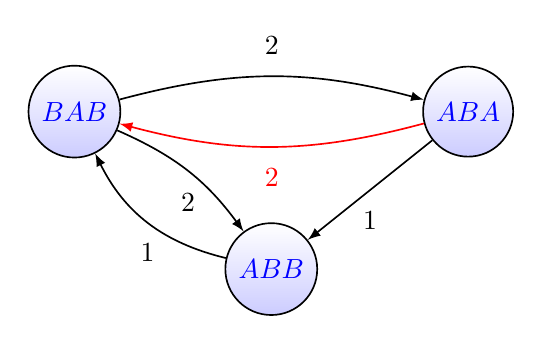
\begin{tikzpicture}[-latex ,auto ,node distance =2 cm and 2.5cm ,on grid ,
semithick ,
state/.style ={ circle ,top color =white , bottom color = blue!20 ,
draw,black , text=blue , minimum width =1 cm}]
\node[state] (C)
{$ABB$};
\node[state] (A) [above left=of C] {$BAB$};
\node[state] (B) [above right =of C] {$ABA$};

\path (C) edge [bend left =25] node[below =0.15 cm] {$1$} (A);
\path (A) edge [bend right = -15] node[below =0.15 cm] {$2$} (C);

\path[color=red] (B) edge [bend  left=15] node[below =0.15 cm] {$2$} (A);
\path (A) edge [bend  right=-15] node[above =0.15 cm] {$2$} (B);
\path (B) edge  node[below =0.15 cm] {$1$} (C);
\end{tikzpicture} 
&    
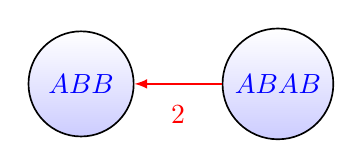
\begin{tikzpicture}[-latex ,auto ,node distance =2 cm and 2.5cm ,on grid ,
semithick ,
state/.style ={ circle ,top color =white , bottom color = blue!20 ,
draw,black , text=blue , minimum width =3.8em}]
\node[state] (A)  {$ABAB$};
\node[state] (B) [left=of A] 
{$ABB$};
\path[color=red] (A) edge node[below=0.15cm]{2} (B);
\end{tikzpicture} 
 & SCS(S)= ABABB \\
 & & length = 5 \\
\hline

\end{tabular}
\end{center}

\vspace{1em}
\begin {center}
\begin{tabular}{|c|c|c|}
\hline
   
   
\SetCell[r=2]{}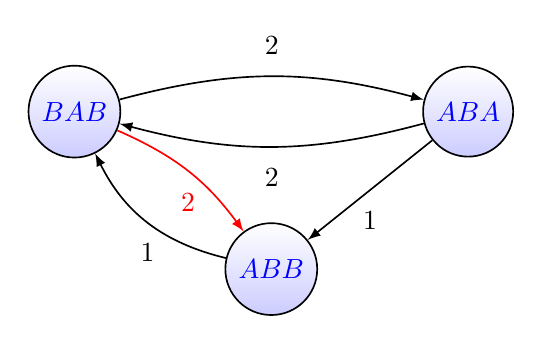
\begin{tikzpicture}[-latex ,auto ,node distance =2 cm and 2.5cm ,on grid ,
semithick ,
state/.style ={ circle ,top color =white , bottom color = blue!20 ,
draw,black , text=blue , minimum width =1 cm}]
\node[state] (C)
{$ABB$};
\node[state] (A) [above left=of C] {$BAB$};
\node[state] (B) [above right =of C] {$ABA$};

\path (C) edge [bend left =25] node[below =0.15 cm] {$1$} (A);
\path[color=red] (A) edge [bend right = -15] node[below =0.15 cm] {$2$} (C);

\path (B) edge [bend  left=15] node[below =0.15 cm] {$2$} (A);
\path (A) edge [bend  right=-15] node[above =0.15 cm] {$2$} (B);
\path (B) edge  node[below =0.15 cm] {$1$} (C);
\end{tikzpicture} 
&    
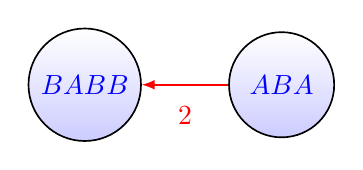
\begin{tikzpicture}[-latex ,auto ,node distance =2 cm and 2.5cm ,on grid ,
semithick ,
state/.style ={ circle ,top color =white , bottom color = blue!20 ,
draw,black , text=blue , minimum width =3.8em}]
\node[state] (A)  {$ABA$};
\node[state] (B) [left=of A] 
{$BABB$};
\path[color=red] (A) edge node[below=0.15cm]{2} (B);
\end{tikzpicture} 
 & SCS(S)= ABABB \\
 & & length = 5 \\
 \hline


\end{tabular}
\end{center}
\vspace{1em}
\textbf{Overall shortest common substring $SCS(S) = ABABB \Rightarrow length =5$ }

\clearpage

\item[c.] Consider the following 3-mer set $S$ = \{CGA, GAT, ATT, TTC, TCT, TTG, TGT, CTA, GTT, TAA, GTA, AAG, AGT\}. Construct the De Bruijn graph, identify an Eulerian walk and reconstruct the corresponding assembly. [5~points]

\vspace{0.5cm}
\textbf{Solution:}\\
Get the 2-mers \\
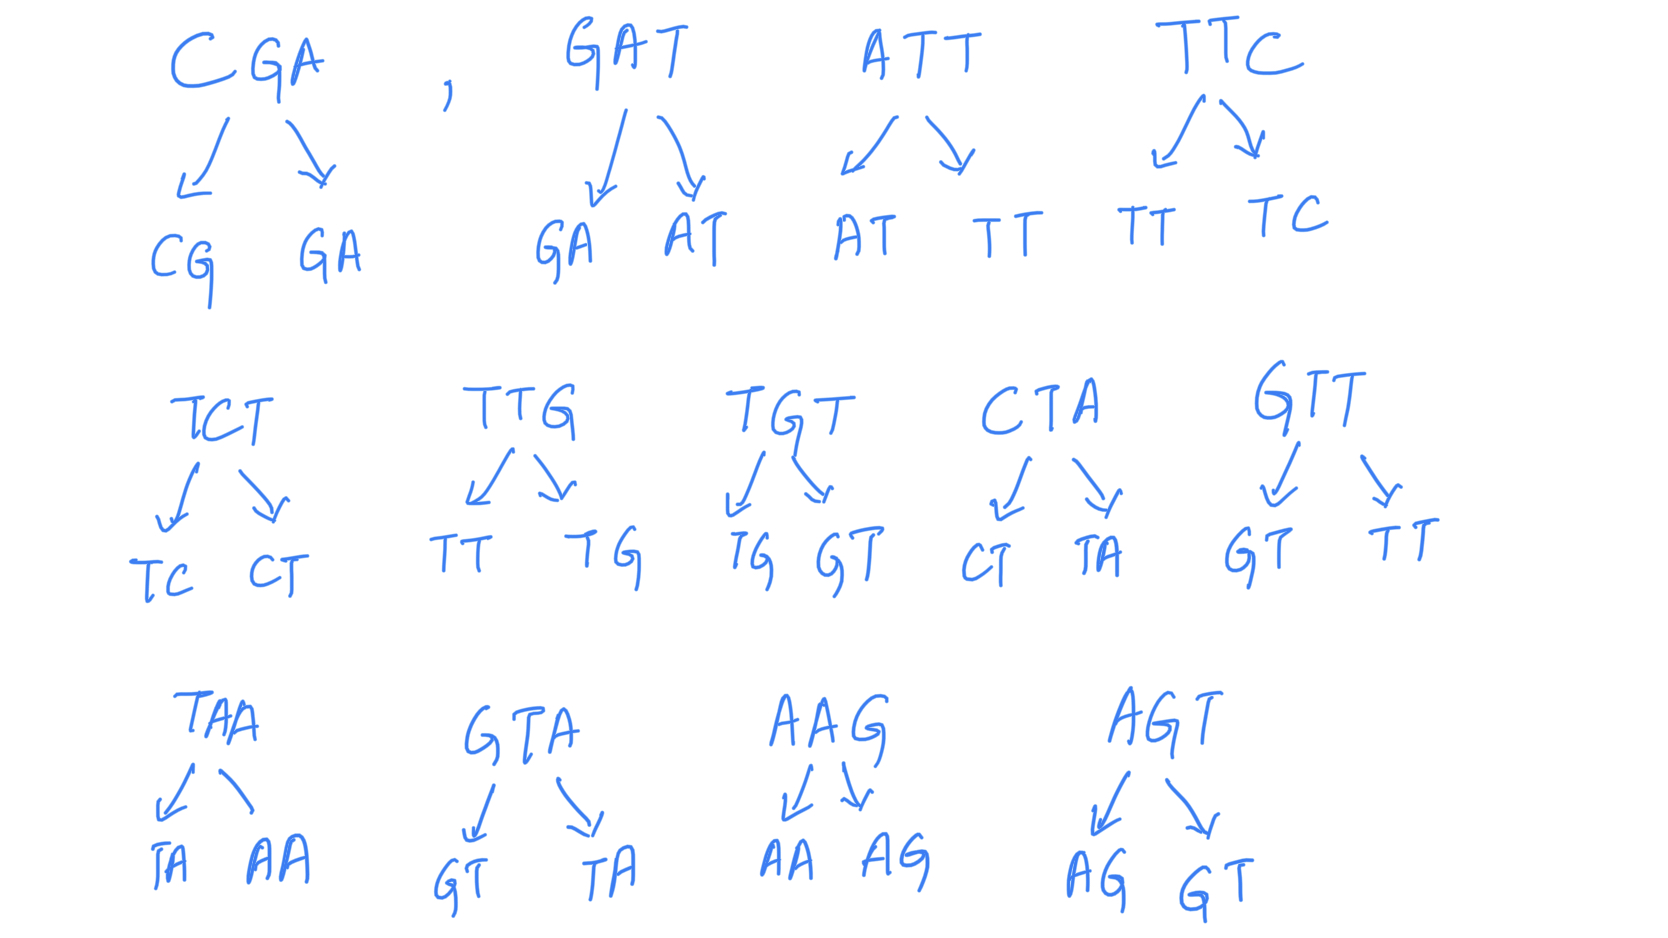
\includegraphics[scale=0.25]{1c1.jpeg}\\

De Bruin Graph \\
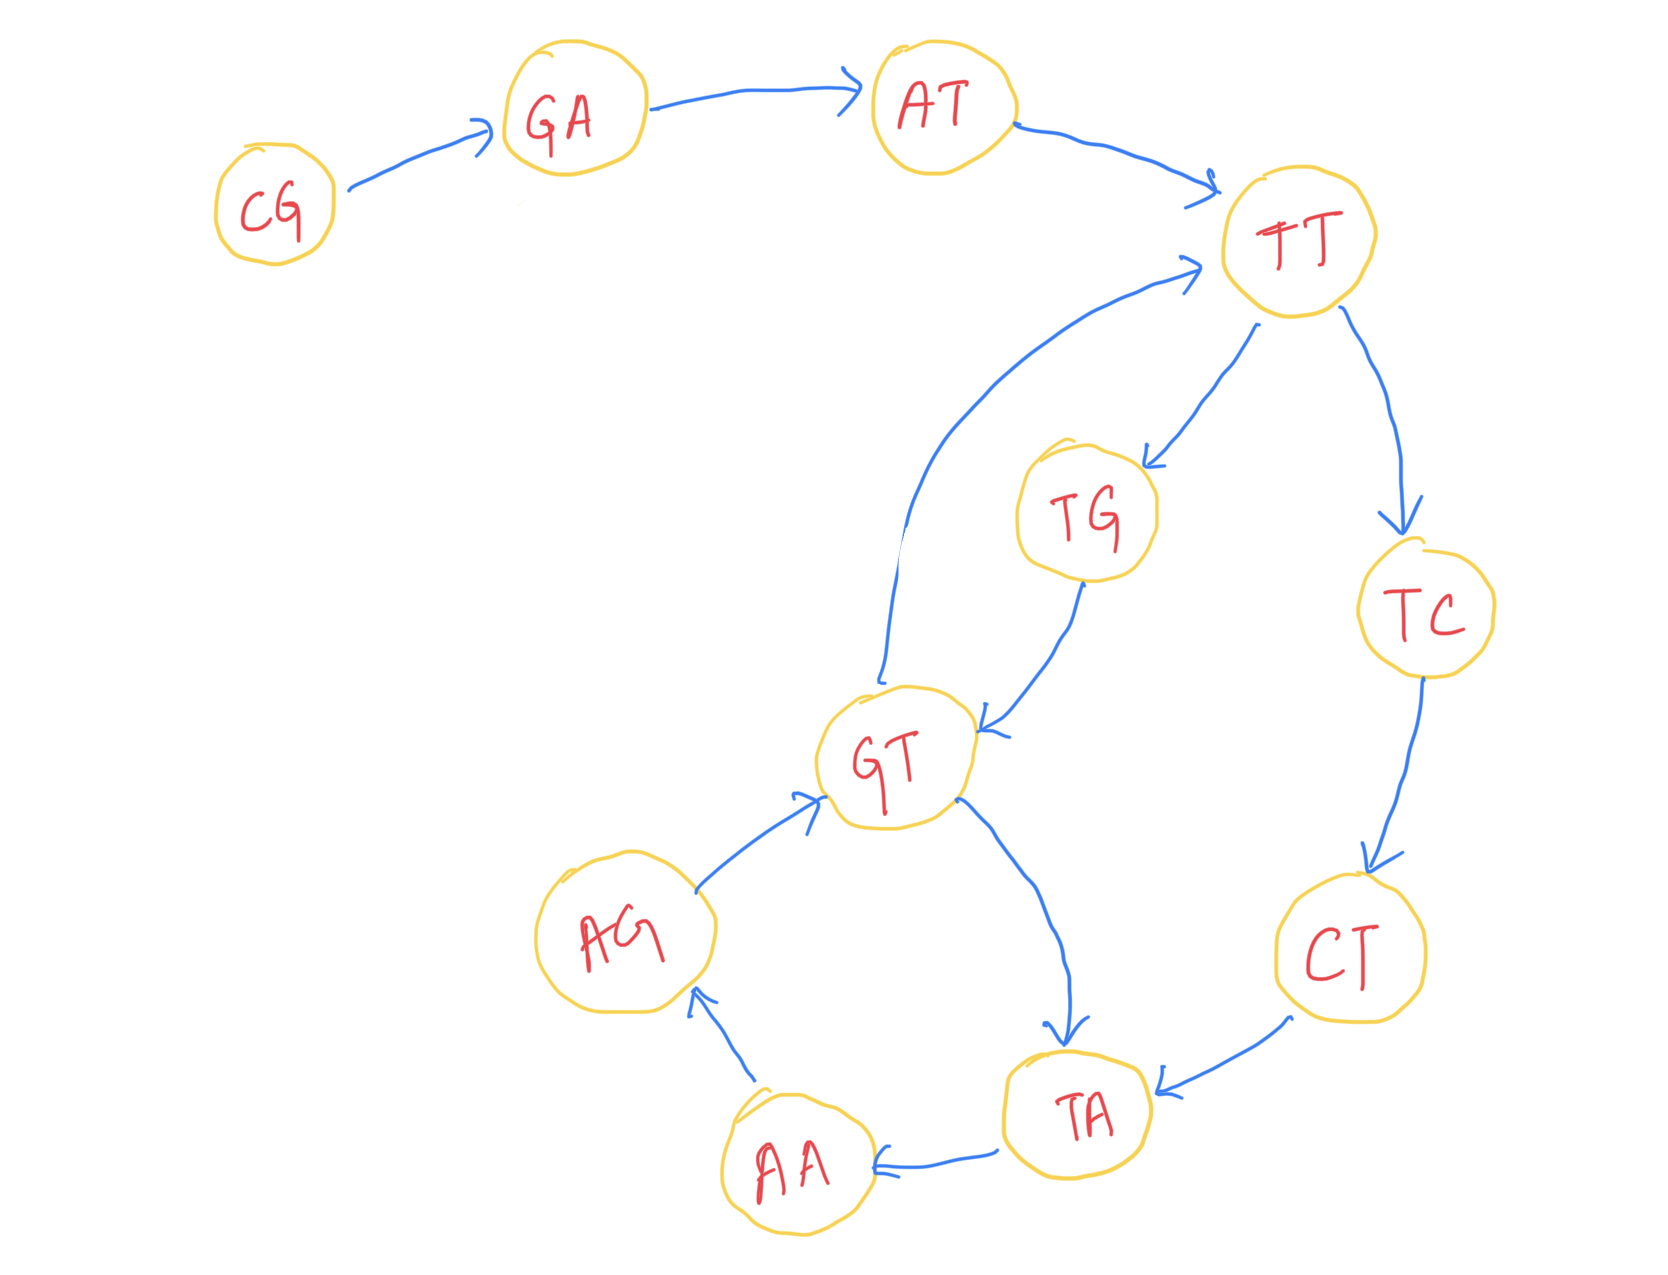
\includegraphics[scale=0.22]{1c2.jpeg}

\textbf{Eulerian Walks :} There are 3 possible solutions 
\begin{enumerate}
    \item $CG\rightarrow GA\rightarrow AT \rightarrow TT \rightarrow TC \rightarrow CT \rightarrow TA \rightarrow AA \rightarrow AG \rightarrow GT \rightarrow TT \rightarrow TG \rightarrow GT \rightarrow TA $ 
    \newline
     \newline
    Final String $\rightarrow$ CGATTCTAAGTTGTA \\

    \item  $CG\rightarrow GA\rightarrow AT \rightarrow TT \rightarrow TG \rightarrow GT \rightarrow TT \rightarrow TC \rightarrow  CT\rightarrow TA \rightarrow AA \rightarrow AG \rightarrow GT \rightarrow TA $ 
     \newline
      \newline
    Final String $\rightarrow$ CGATTGTTCTAAGTA \\

    \item  $CG\rightarrow GA\rightarrow AT \rightarrow TT \rightarrow TG \rightarrow GT \rightarrow TA \rightarrow AA \rightarrow  AG\rightarrow GT \rightarrow TT \rightarrow TC \rightarrow CT \rightarrow TA $ 
     \newline
     \newline
    Final String $\rightarrow$ CGATTGTAAGTTCTA
\end{enumerate}

\vspace{1cm}

\end{enumerate}
\newpage
\begin{enumerate}
\item[2.] \textbf{Assembly II} [25 points]

Suppose you have the following set of sequenced reads $R = \{\texttt{GTACTG, ACTTGT} \}. $

\begin{enumerate}
\item[a.]  Draw the De Bruijn graph for this set of reads with $k=4$. [5~points] \\

\textbf{Solution:}\\
Get the 4-mers and split into left and right 3-mers\\
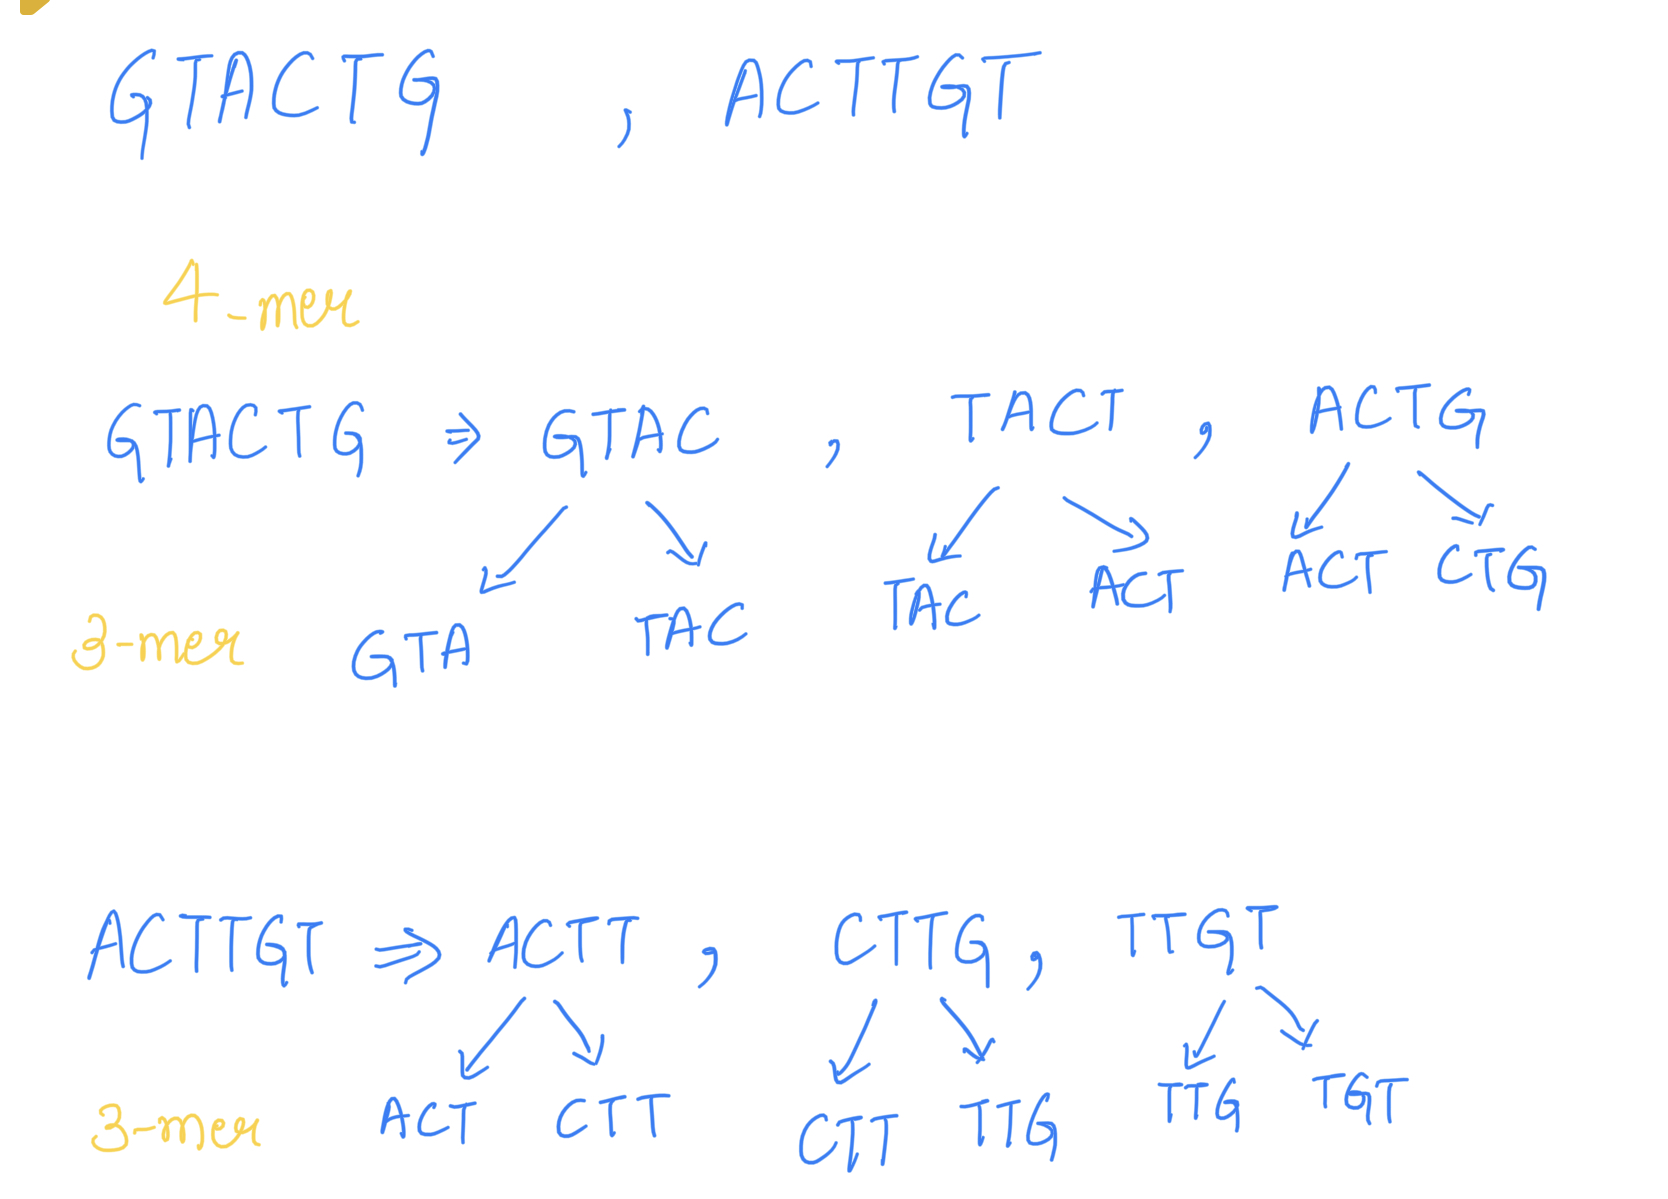
\includegraphics[scale=0.2]{2a1.jpeg}\\
\newline
Build the De Bruijn Graph \\
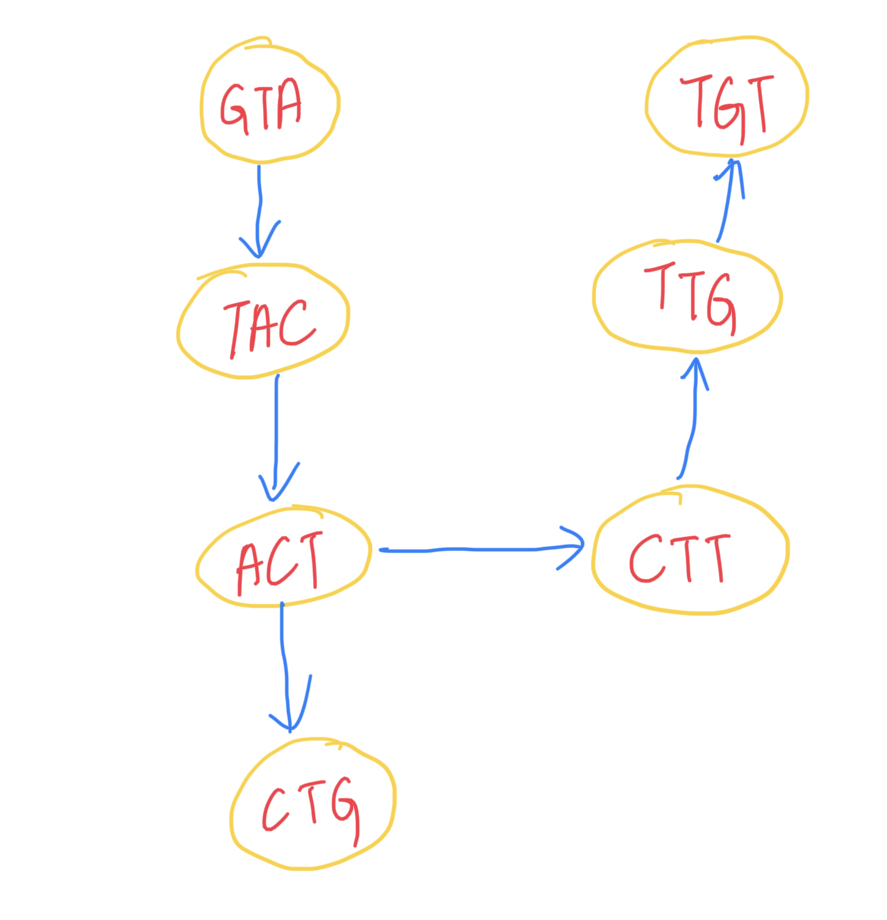
\includegraphics[scale=0.2]{2a2.jpeg}\\
\newpage

\item[b.] Does a Eulerian walk exist in the graph your drew?  If so, give the complete sequence it indicates for the underlying genome (or one if multiple Eulerian paths exist).  If not, explain why not. [5~points]

\fbox{\parbox{\linewidth}{
\vspace{1cm}
A Node in graph is semi-balanced if indegree differs from outdegree by 1\\

We know that a directed, connected graph is Eulerian if
and only if it has at most 2 semi-balanced
nodes and all other nodes are balanced \\ 
\newline
In 2a, the De Bruijn Graph  has 3 semi-balanced nodes GTA, ACT, TGT. Hence it doesn't have a Eulerian walk .

\vspace{10cm}
}}
\newpage
\item[c.]  Draw the De Bruijn graph for this set of reads with $k=3$. [10~points]
\vspace{1cm}
\textbf{Solution:}\\
Get the 3-mers and split into left and right 2-mers\\
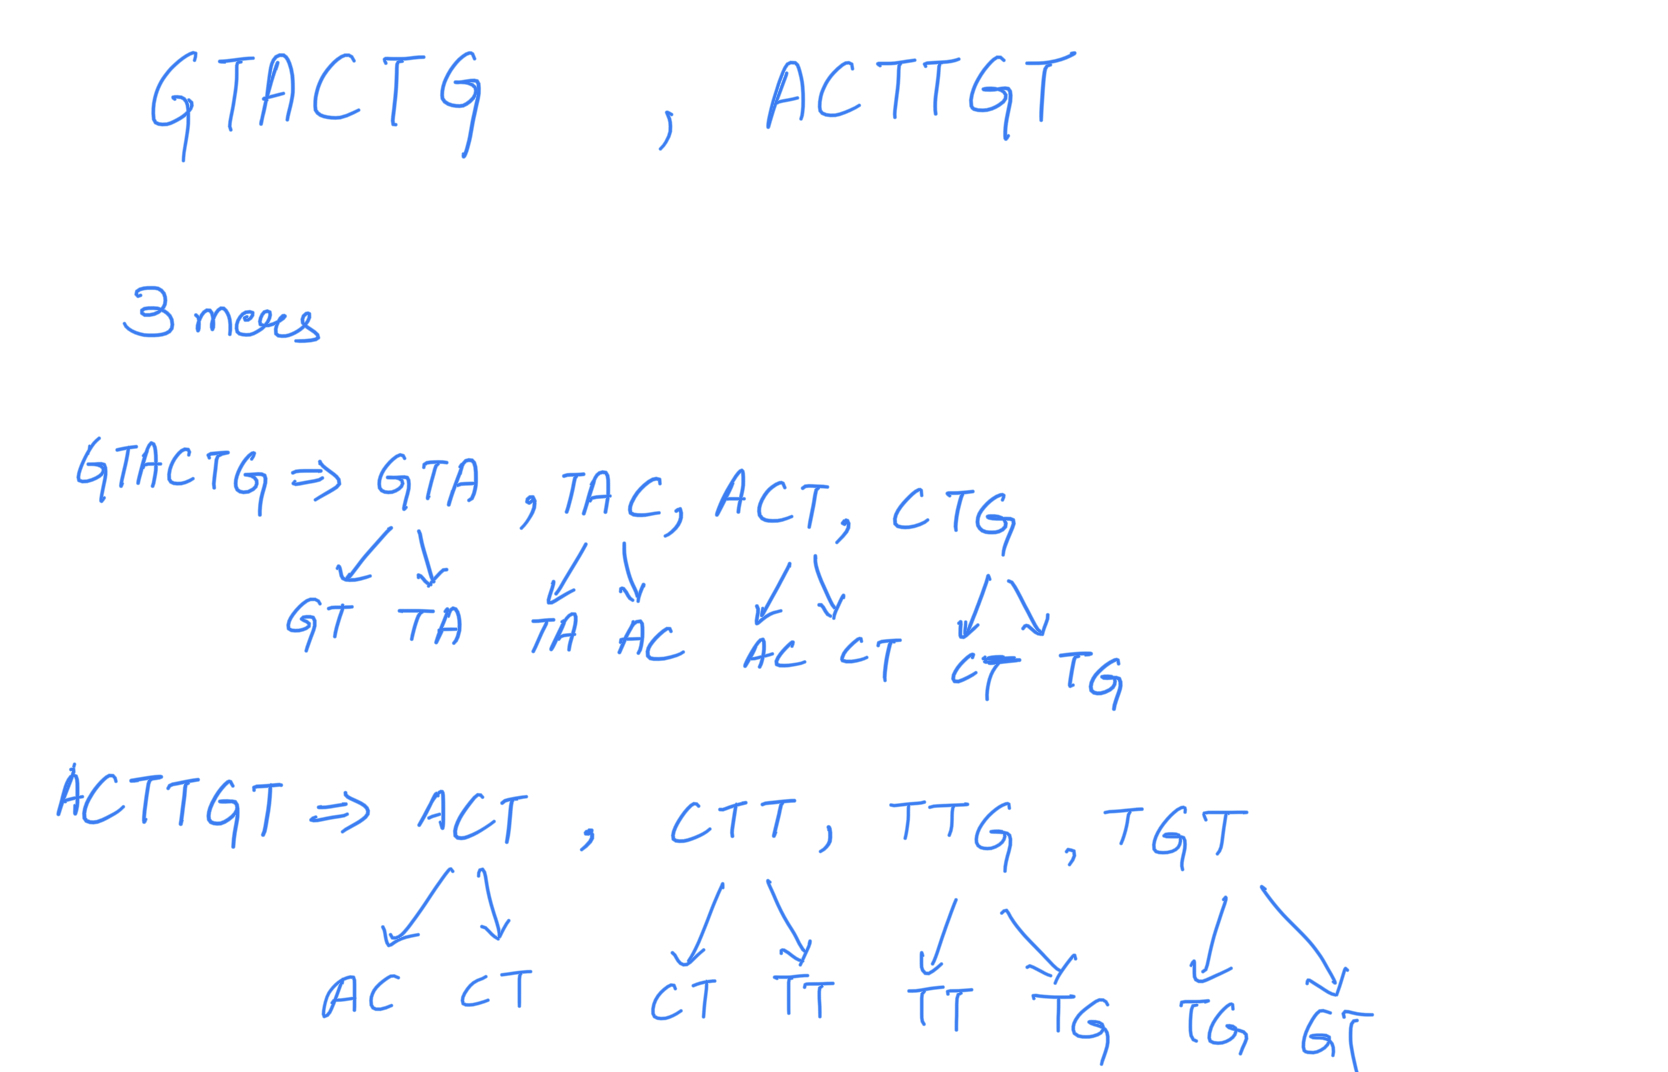
\includegraphics[scale=0.23]{2c1.jpeg}
\newline
Build the De Bruijn Graph \\
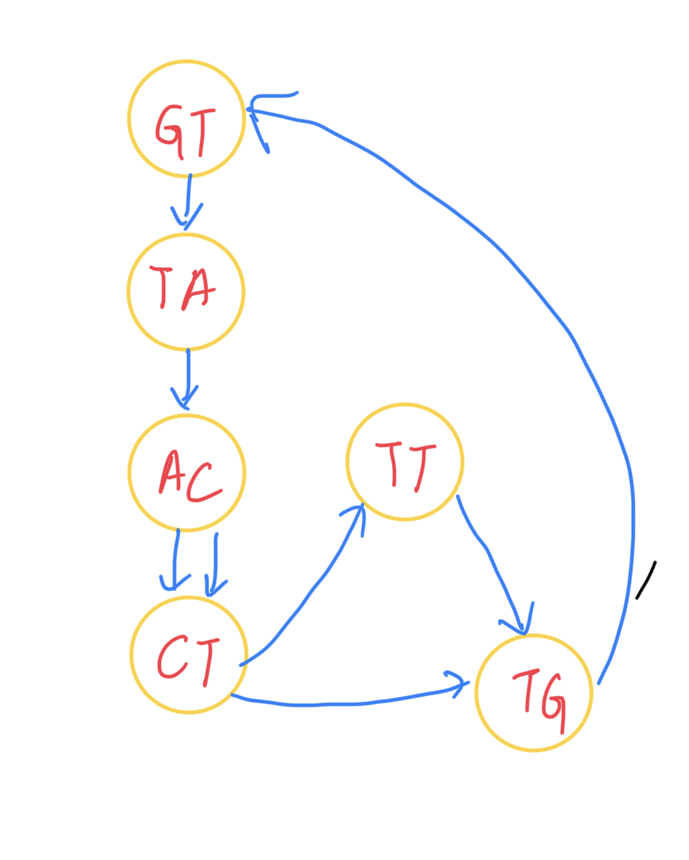
\includegraphics[scale=0.2]{2c2.jpeg}
\newpage
\item[d.] Does a Eulerian walk exist in the graph your drew?  If so, give the complete sequence it indicates for the underlying genome (or one such sequence if multiple Eulerian paths exist).  If not, explain why not. [5~points]

\fbox{\parbox{\linewidth}{
\vspace{1cm}
Since the De Bruin Graph in 2c has exactly two semibalanced nodes - AC and TG, there exists a Eulerian Walk in the graph. \\
We can have two following sequences \\

\begin{enumerate}
    \item $AC\rightarrow CT\rightarrow TT \rightarrow TG \rightarrow GT \rightarrow TA \rightarrow AC \rightarrow CT \rightarrow TG  $ 
    \newline
     \newline
    Final String $\rightarrow$ ACTTGTACTG \\

 \item $AC\rightarrow CT \rightarrow TG \rightarrow GT \rightarrow TA \rightarrow AC \rightarrow CT \rightarrow TT \rightarrow TG  $ 
    \newline
     \newline
    Final String $\rightarrow$ ACTGTACTTG \\

\end{enumerate}

\vspace{5cm}
}}

\end{enumerate}
\end{enumerate}
\end{enumerate}

\end{document}
